For now, consider the easier case where no additional surgery is carried out on the Bourgeois manifold.
That makes the proof for the homological obstruction theorem easier to understand.
It can be generalized to the case with surgery, but this is omitted here.
The idea is to cap off both sides (i.e. $V_+$ and $V_-$) of the convex decomposition
using the surgery procedure introduced in the last section.
Topologically, this will result in a cobordism from $M\times T^2$ to $\Gamma \times S^2$.

In \cite[Section 6]{MNW13}, where blowdown surgery of a Giroux domain is first introduced,
it is shown that it corresponds to a symplectic cobordism.
The setting there is actually more general: The authors consider a Giroux
domain where already some of the boundary components have been blown down.
In this case, the situation is simpler: The Giroux domain 
$V_\pm \times S^1 \subset V \times S^1 = M \times T^2$
is directly obtained from the corresponding ideal Liouville domain $V_\pm$ by 
round contactization.
Its boundary is given by 
\[
    \partial V_\pm \times S^1 = \Gamma \times S^1.
\]

Now, considering the manifold $(V_+ \cup_\Gamma V_-)\times S^1$, perform a blowdown
surgery on both ends, i.e. remove the interior of $V_\pm \times S^1$ and blow down the boundary $\Gamma \times S^1$.
In order to do this properly, it is necessary to consider a neighborhood 
$\Gamma \times (-\delta, \delta)$ around the dividing set and 
instead of $V_\pm$ take $V_\pm' \coloneqq V_\pm \setminus \Gamma \times [0, \pm \delta]$.
Topologically, blowing down $\Gamma \times S^1$ yields $\Gamma \times D^2$.
As this is done on both sides, the result is 
\[
    \Gamma \times D^2 \cup_{\Gamma \times S^1 \times -\delta} \Gamma \times (-\delta,\delta) 
    \cup_{\Gamma \times S^1 \times +\delta} \Gamma \times D^2 \cong \Gamma \times S^2.
\]
For an example, see \cref{fig:cap_cobordism}.

\begin{figure}[ht]
    \begin{subfigure}[t]{.54\linewidth}
        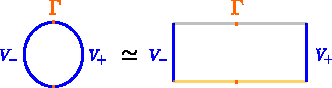
\includegraphics[trim=-.3cm -.5cm -.3cm -.5cm, width=\linewidth]{../images/convex_decomposition_of_s1.pdf}
        \subcaption{The convex decomposition of $V = S^1$ 
        where the dividing set $\Gamma$ consists of two points is homotopic to a rectangle.}
    \end{subfigure}\hspace*{.1\linewidth}
    \begin{subfigure}[t]{.35\linewidth}
        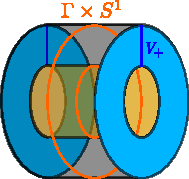
\includegraphics[trim=-.5cm -.5cm -.5cm -.5cm, width=\linewidth]{../images/v_times_s1.pdf}
        \subcaption{Taking the product with $S^1$ yields $V \times S^1$, in this case a torus.}
    \end{subfigure}
    \begin{subfigure}{.9\linewidth}
        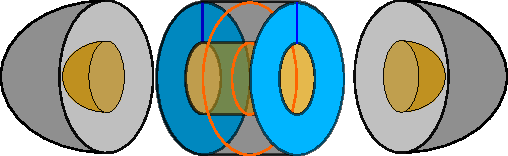
\includegraphics[trim=-.5cm -.5cm -.5cm -.5cm, width=\linewidth]{../images/v_times_s1_with_caps.pdf}
        \subcaption{On the upper boundary of the capping cobordism, one adds $V_\pm \times D^2$-caps to the torus.}
    \end{subfigure}
    \begin{subfigure}{.9\linewidth}
        \centering
        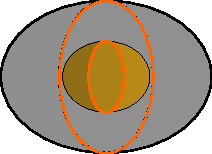
\includegraphics[trim=-.5cm -.5cm -.5cm -.5cm, width=.5\linewidth]{../images/gamma_times_s2.pdf}
        \subcaption{As a result, the upper boundary of the cobordism is $\Gamma \times S^2$. In this case that amounts to an outer (gray) and an inner (yellow) sphere.}
    \end{subfigure}
    \caption[short]{A low dimensional sketch for the upper boundary of the capping cobordism.}
    \label{fig:cap_cobordism}
\end{figure}

This whole surgery procedure can be realized as applying a certain symplectic cobordism.
This is made precise in the following
\begin{lemma}(follows from \cite[Theorem 6.1]{MNW13}, cf. \cite[Lemma 6.1]{BGM22})\label{lem:capping_cobordism}
    There is a symplectic cobordism $(C, \omega)$ with negative (i.e. concave) 
    contact boundary $\partial_-C = V \times S^1$ and weakly convex positive boundary
    $\partial_+ C = \Gamma \times S^2$ where $\Gamma = \partial V$. 
    Moreover, there is a tubular neighborhood $(-\delta, 0] \times \partial_+ C$
    such that $\omega$ is of the form $d(e^t \alpha_\Gamma) + \omega_S$, 
    where $t \in (-\delta, 0]$ and 
    \begin{itemize}
        \item $\omega_S$ is an area form on $S^2$,
        \item $\alpha_\Gamma$ is a contact form on $\Gamma$.
    \end{itemize}
    Lastly, there are symplectic submanifolds $C_\pm$ , diffeomorphic to $V_\pm$, 
    such that $C\setminus C_\pm$ deformation retracts onto its negative boundary, 
    and such that $C_\pm$ intersect transversely, positively and in exactly one point, 
    each symplectic sphere in the previously described neighborhood 
    of the positive boundary $\partial_+ C$.
\end{lemma}

The submanifolds $C_\pm$ are basically $V_\pm \times 0 \subset V_\pm \times D^2$, i.e. 
the co-cores of the attached handles.
If these submanifolds are taken out, the effect of the capping is topologically trivial.
Therefore, the remaning cobordism is topologically just $\partial_- C\times [0,1]$.
This clearly deformation retracts to the negative boundary.
One can also construct a slightly modified deformation retract where instead 
of removing the co-cores, one removes slight push-offs 
(i.e. submanifolds that are obtained by shifting $C_\pm$ aside by a section of its normal bundle).
Then, $C_\pm$ retracts to $V_\pm$.